%%%%%%%%%%%%%%%%%%%%%%%%%%%%%%%%%%%%%%%%%%%%%%%%%%%%%%%
% % Lines starting with % are comments, which are ignored.
% % This is a handy way of indicating the date and version of
% % your document, to wit:
% %
% % LaTeX sample file
% % Modified March, 2002
% %
%%%%%%%%%%%%%%%%%%%%%%%%%%%%%%%%%%%%%%%%%%%%%%%%%%%%%%%
\DocumentMetadata{
  % PDF standards: ONE key whose value is a comma-separated list --
  % UA-2 (accessibility) plus A-4f (archival; the archival companion of
  % UA-2). Do NOT use separate pdfstandard=... keys: with ordinary
  % key-value parsing only the last one takes effect.
  pdfstandard={UA-2,A-4f},
  lang=en-US,
  tagging=on,
  tagging-setup={
    math/setup=mathml-SE
  }
}

\documentclass{ltx-talk}
% lecture-macros.tex -- shared package setup for lecture-template.tex
% (ltx-talk slides / handouts).
%
% NOTE ON PATHS: every template in this repository is stored one level up
% from where it is compiled (see README.md). All relative \input paths
% below are resolved against the folder the document is compiled in,
% which sits one directory above this file.

% --- Tables, bookmarks, strikethrough ------------------------------------
% booktabs: professional table rules (\toprule, \midrule, \bottomrule)
% bookmark: PDF outline entries (PDF bookmarks)
% ulem[normalem]: \sout strikethrough that survives math mode
\usepackage{booktabs}
\usepackage{bookmark}
\usepackage[normalem]{ulem}
\usepackage{multicol}

% --- Math ------------------------------------------------------------
% amsmath: equation environments and numbering
% mathrsfs: \mathfrak  |  stmaryrd: extra symbols
\usepackage{amsmath}
\usepackage{mathrsfs}
\usepackage{stmaryrd}

% --- Layout -------------------------------------------------------------
% float: [H] float placement
% fontspec: Unicode/OpenType fonts (compile with XeLaTeX or LuaLaTeX)
\usepackage{float}
\usepackage{fontspec}

% --- Colors ---------------------------------------------------------------
% dvipsnames: extended named color palette (the Accessible* colors below
% are built on it);
% table: \rowcolors / \cellcolor for shading tables.
% NOTE: xcolor may only be loaded ONCE per document -- a second
% \usepackage{xcolor} with different options is a fatal "Option clash"
% error, so ALL of its options are listed here.
\usepackage[dvipsnames,table]{xcolor}

% --- Multimedia -----------------------------------------------------------
% animate: embeds audio/video (and legacy Flash) media in a frame.
\usepackage{animate}

% --- Bibliography ----------------------------------------------------------
% biblatex (biber backend): citations for lecture notes.
\usepackage[
  backend=biber,
  style=alphabetic,
  url=true,
  doi=true,
  isbn=true,
  backref=true
]{biblatex}

% --- Colored boxes ----------------------------------------------------------
% talkthemetcolorbox: the colored-box theme for ltx-talk slides
% (shadow/rounded/shaded blocks, showtitle, titlepage styles).
\usepackage[
  shadow,
  rounded,
  shaded,
  blocks,
  showtitle,
  titlepage
]{talkthemetcolorbox}

% --- "theindex" helper environment ------------------------------------------
% Provides a lightweight theindex environment (an itemize) and the
% \@idxitem/\subitem/\subsubitem/\indexspace macros that LaTeX's standard
% theindex machinery expects, so hand-written index pages indent correctly.
\makeatletter
\newenvironment{theindex}
  {\begin{itemize}}
  {\end{itemize}}
\providecommand\@idxitem{\par\hangindent 40\p@}
\providecommand\subitem{\@idxitem \hspace*{20\p@}}
\providecommand\subsubitem{\@idxitem \hspace*{30\p@}}
\providecommand\indexspace{\par \vskip 10\p@ \@plus5\p@ \@minus3\p@\relax}
\makeatother

% --- Index -----------------------------------------------------------------
% imakeidx: builds the printed index.
% The redefinition below appends "|hyperpage" to every index entry so that,
% in the PDF, each index entry is a link to its page.
\usepackage{imakeidx}
\makeatletter
\let\imki@orig@wrindexentrysplit\imki@wrindexentrysplit
\renewcommand\imki@wrindexentrysplit[3]{%
  \imki@orig@wrindexentrysplit{#1}{#2|hyperpage}{#3}%
}

\makeatletter
% --- Section titles: capture + one bookmark per logical section -------------
% \section is redefined so that:
%   1. the section title is captured into the plain-TeX register
%      \mytalksectitletoks (reprinted verbatim on the auto divider frame,
%      see the cmd/section/after hook below -- plain-TeX storage is
%      catcode-safe, unlike expanding the title in a hook), and
%   2. exactly ONE depth-1 PDF bookmark is created per \section call
%      (hyperref's own bookmark is suppressed via \Hy@writebookmark).
\DeclareCommandCopy{\OriginalSectionForBookmarks}{\section}
\newtoks\mytalksectitletoks

\RenewDocumentCommand{\section}{s o m}{%
  \begingroup
    \def\Hy@writebookmark##1##2##3##4##5{}%
    \global\mytalksectitletoks={#3}%
    \IfBooleanTF{#1}
      {\phantomsection\IfNoValueTF{#2}{\OriginalSectionForBookmarks*{#3}}{\OriginalSectionForBookmarks*[#2]{#3}}}%
      {\IfNoValueTF{#2}{\OriginalSectionForBookmarks{#3}}{\OriginalSectionForBookmarks[#2]{#3}}}%
  \endgroup
  \IfBooleanTF{#1}
    {\IfNoValueTF{#2}{\pdfbookmark[1]{#3}{section-star.\thepage.\number\inputlineno}}{\pdfbookmark[1]{#2}{section-star.\thepage.\number\inputlineno}}}%
    {\IfNoValueTF{#2}{\pdfbookmark[1]{Section \thesection: #3}{section.\thesection}}{\pdfbookmark[1]{Section \thesection: #2}{section.\thesection}}}%
}
\makeatother

% --- One PDF bookmark per logical frame (NOT per overlay) ---------------------
% ltx-talk writes one PDF page per overlay, so a naive frametitle hook would
% register a new bookmark for every overlay of the same frame. The
% \g_slideutils_frame_bookmark_int register remembers the last frame that
% got a bookmark, so subsequent overlays of the same frame are skipped.
% This is also what keeps BeamerPresenter's cumulative annotations working:
% one logical frame must stay one logical unit in the PDF outline.
\ExplSyntaxOn
\int_new:N \g_slideutils_frame_bookmark_int

\AddToHook{cmd/frametitle/after}{%
  \tl_if_empty:NF \g__talk_frame_title_tl
    {
      \ifnum\value{frame}=\g_slideutils_frame_bookmark_int\relax
      \else
        \int_gset:Nn \g_slideutils_frame_bookmark_int { \value{frame} }%
        \pdfbookmark[2]{\tl_use:N \g__talk_frame_title_tl}
          {frame.\int_use:N \g_slideutils_frame_bookmark_int}
      \fi
    }
}
\ExplSyntaxOff
\makeatother

% --- Printed index + theme for the colored boxes -------------------------------
% \makeindex[...]: two-column index titled "Index", listed in the TOC.
% The two EditInstance calls style the standard header/footer instances
% of talkthemetcolorbox (cyan background; footer order title/author/
% date/framenumber).
\makeindex[columns=2, title=Index, intoc]\EditInstance{header}{std}{
  background-color = cyan,
  color            = black,
  height           = 0.75cm
}
\EditInstance{footer}{std}{
  background-color = cyan,
  element-order = {title, author, date, framenumber},
}

% --- Auto section divider frame ---------------------------------------------------
% After each \section, insert a centered, large, structure-colored frame
% that prints the section title (from \mytalksectitletoks).
\AddToHook{cmd/section/after}{%
  \begin{frame}
    \centering
    \color{structure}
    \LARGE
    \the\mytalksectitletoks
  \end{frame}%
}

% --- Tagging sockets (tagged PDF structure) ---------------------------------------
% ltx-talk exposes tagging "sockets" where the PDF structure can attach
% section titles; register one and leave it unassigned (none) so the
% class's own tagging keeps control.
\ExplSyntaxOn
\AtBeginDocument{
  \NewTaggingSocketPlug { talk / sec / title } { none } { }
  \AssignTaggingSocketPlug { talk / sec / title } { none }
}
\ExplSyntaxOff

% --- Accessibility roles ----------------------------------------------------------------
% Map \frametitle to the H1 heading role in the tagged PDF, so screen
% readers treat slide titles as headings.
\tagpdfsetup{role / new-tag = frametitle / H1}

\makeatletter
% --- Page label = frame number -------------------------------------------------------
% Redefine what feeds the PDF page label to track the frame counter,
% not the physical page counter. Replace \theframenumber below with
% whatever internal macro/property ltx-talk actually uses to produce
% the "framenumber" footer element — confirm via ltx-talk-frame.dtx.
\renewcommand\thepage{\arabic{frame}}
\makeatother

\addbibresource{refs.bib}

% --- "Problem Time!" slides ------------------------------------------------------------------
% \ProblemSlide{problem}{solution} emits two frames: the problem, then
% its solution after a \pause, each numbered by the problem counter.
\newcounter{problemcounter}
\setcounter{problemcounter}{0}
\newcommand{\ProblemSlide}[2]{
  \stepcounter{problemcounter}
  \begin{frame}
    \frametitle{Problem Time!}
    Problem \theproblemcounter: #1
  \end{frame}

  \begin{frame}
    \frametitle{Problem Time!}
    Solution to Problem \theproblemcounter: \pause

    #2
  \end{frame}
}
% \highlight[<colour>]{<stuff>}
% from https://tex.stackexchange.com/questions/33401/a-version-of-colorbox-that-works-inside-math-environments
\newcommand{\highlight}[2][yellow]{\mathchoice%
  {\colorbox{#1}{$\displaystyle#2$}}%
  {\colorbox{#1}{$\textstyle#2$}}%
  {\colorbox{#1}{$\scriptstyle#2$}}%
  {\colorbox{#1}{$\scriptscriptstyle#2$}}}%

% --- Fonts ------------------------------------------------------------------------------
% Lato (text) + LeteSansMath (math): open, accessible typefaces.
\setmainfont{Lato}[
  Ligatures=TeX,
  Numbers={Lining,Monospaced}
]
\setsansfont{Lato}[
  Ligatures=TeX,
  Numbers={Lining,Monospaced}
]
\setmathfont{LeteSansMath.otf}\usepackage{emoji}

% --- Accessible colors ---------------------------------------------------------------------
% WCAG-contrast-safe variants of red/green for text on white:
% red!80!black and green!40!black both clear the 4.5:1 requirement.
% AltYellow: soft background for highlight boxes.
\colorlet{AccessibleRed}{red!80!black}
\colorlet{AccessibleGreen}{green!40!black}
\definecolor{AltYellow}{RGB}{255,245,170}

% --- Links ---------------------------------------------------------------------------------
% hyperref + link colors: every link uses AccessibleGreen (7.2:1 on
% white), so internal, citation, and URL links all pass WCAG 1.4.3.
\usepackage{hyperref}
\hypersetup{
  colorlinks=true,
  linkcolor=AccessibleGreen,
  urlcolor=AccessibleGreen,
  citecolor=AccessibleGreen,
}

% --- Shared course macros ---------------------------------------------------------------------
% Root macros.tex: math shorthands used across all course documents
% (\RR, \NN, \ZZ, \QQ, \grad, \curl, \tr, \der, \pder, ...).
\newcommand{\RR}{\mathbb{R}}
\newcommand{\NN}{\mathbb{N}}
\newcommand{\ZZ}{\mathbb{Z}}
\newcommand{\QQ}{\mathbb{Q}}
\newcommand{\vv}{\vec{v}}
\newcommand{\ww}{\vec{w}}
\newcommand{\xx}{\vec{x}}
\newcommand{\yy}{\vec{y}}
\newcommand{\zz}{\vec{z}}
\newcommand{\uu}{\vec{u}}
\newcommand{\basis}[1]{\vec{e_{#1}}}
\newcommand{\id}{\mathrm{id}}
\newcommand{\CC}{\mathbb{C}}
\renewcommand{\div}{\operatorname{div}}
\newcommand{\grad}{\operatorname{grad}}
\newcommand{\curl}{\operatorname{curl}}
\newcommand{\tr}{\operatorname{tr}}
\newcommand{\der}[2]{\dfrac{d #1}{d #2}}
\newcommand{\pder}[3][]{\dfrac{\partial^{#1} #2}{\partial #3}}


% % Title and author(s)
%%%%%%%%%%%%%%%%%%%%%%%%%%%%%%%%%%%%%%%%%%%%%%%%%%%%%%%
\title{Lecture 5 - The Derivative}
\author{Garrett Credi}
\date{09/22/26}
%%%%%%%%%%%%%%%%%%%%%%%%%%%%%%%%%%%%%%%%%%%%%%%%%%%%%%%
% %
% % The next command allows your in import encapsulated
% % postscript files, .epsf or .eps files, which
% % contain vector graphic image data.
% %
%%%%%%%%%%%%%%%%%%%%%%%%%%%%%%%%%%%%%%%%%%%%%%%%%%%%%%%
% %   The first thanks indicates your affiliation
% %
% %  Just the name here.
% %
% % Your mailing address goes at the end.
% %
% % \thanks is also how you indicate grant support
% %
%%%%%%%%%%%%%%%%%%%%%%%%%%%%%%%%%%%%%%%%%%%%%%%%%%%%%%%

%%%%%%%%%%%%%%%%%%%%%%%%%%%%%%%%%%%%%%%%%%%%%%%%%%%%%%%
% $ The next command ensures the margins are 1 inch on
% % all sides.
% %
%%%%%%%%%%%%%%%%%%%%%%%%%%%%%%%%%%%%%%%%%%%%%%%%%%%%%%%
\begin{document}
\begin{frame}
  \maketitle
\end{frame}

\begin{frame}
  \frametitle{Homework Updates/Info/Yappery?}

  After reading the engagement portfolios, I just had a few things I thought might be useful to say: \pause

  \begin{enumerate}
    \item For choosing problems - I'd recommend looking over each of the problem types and choosing \textit{a few problems from many problem types}. \pause
    \item Come review time (for quizzes and exams) the other problems you did not solve will be very useful practice problems \pause (homework's will be uploaded on Canvas since evil gradescope doesn't let you see them after the due date) \pause
    \item If you're choosing homework problems in a way that's making you feel lost or making you feel unprepared for the quizzes please talk to me so we can discuss different strategies :)
  \end{enumerate}
\end{frame}

\begin{frame}
  \frametitle{Quiz Time!}

  Let's get into nice orderly rows, spread out as much as possible, and slay this quiz :)
\end{frame}

\begin{frame}
  \frametitle{The Road So Far}

  So far we've developed this notion of a limit: \pause
  \begin{enumerate}
    \item Limits $\lim\limits_{x \rightarrow a} f(x)$ \pause are \textit{the values that $f(x)$ approximates as $x$ approximates $a$ to closer and closer degrees} \pause
    \item Functions whose \textit{actual} values 
      match their approximated values at $x = a$ \pause 
      (e.g. where $f(a) = \lim\limits_{x \rightarrow a} f(x)$) 
      are called \pause \textit{continuous at $x = a$}. 
      \pause c.f. continuous on $[a,b]$, and continuous \pause
    \item We developed \textit{maaaany} different tools to compute limits. 
  \end{enumerate}
\end{frame}

\begin{frame}
  \frametitle{Constant Value Approximation}

  For a function $f(x)$ that is \textit{continuous at $x = a$}, \pause 
  how good is the approximation $f(x) \approx f(a)$ when $a \approx x$? \pause

  \begin{columns}[t]
    \begin{column}{0.48\textwidth}
      \pause
      \begin{figure}
        \centering
        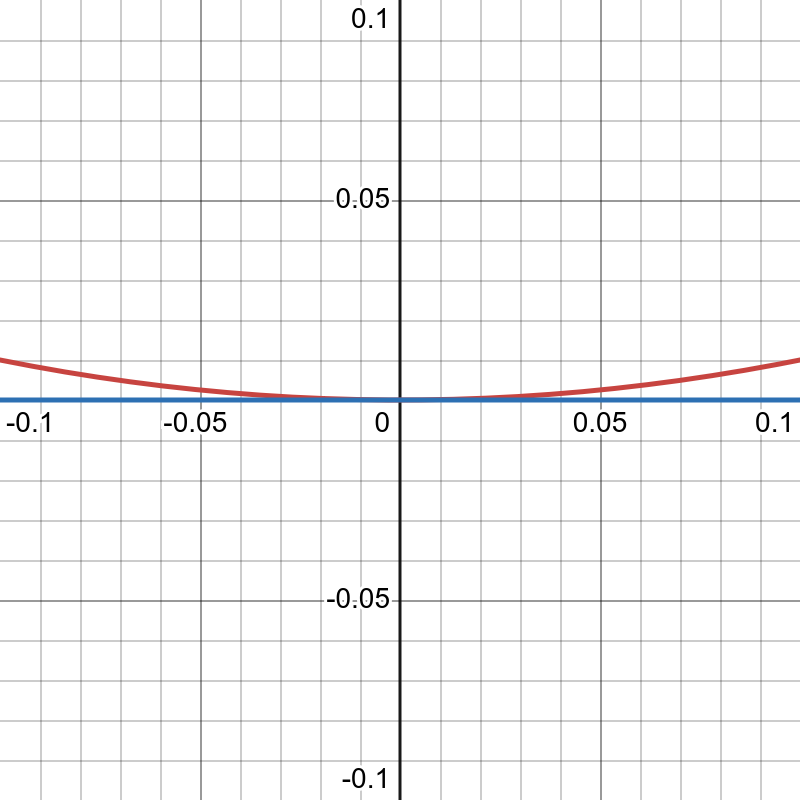
\includegraphics[height=0.3\textheight]{x_squared_graph.png}
        \caption{The graph of $f(x) = x^2$ near $x = 0$}
      \end{figure}
    \end{column}
    \begin{column}{0.48\textwidth}
      \pause
      \begin{figure}
        \centering
        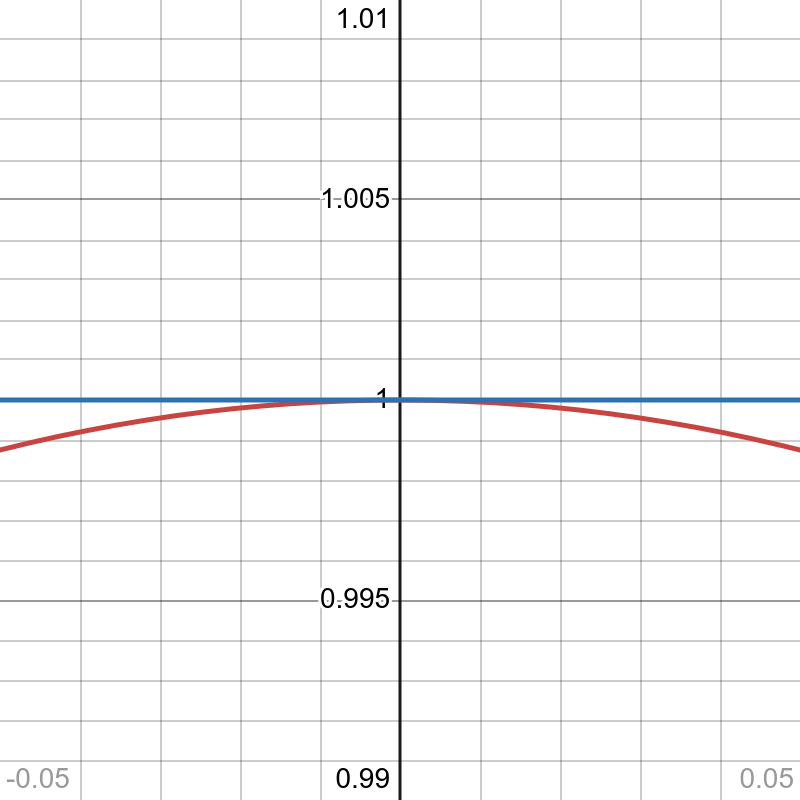
\includegraphics[height=0.3\textheight]{cos_x_graph.png}
        \caption{The graph of $f(x) = \cos(x)$ near $x = 0$}
      \end{figure}
    \end{column}
  \end{columns}
  % ---- bottom row ----
  \begin{columns}[t]
    \begin{column}{0.48\textwidth}
      \pause
      \begin{figure}
        \centering
        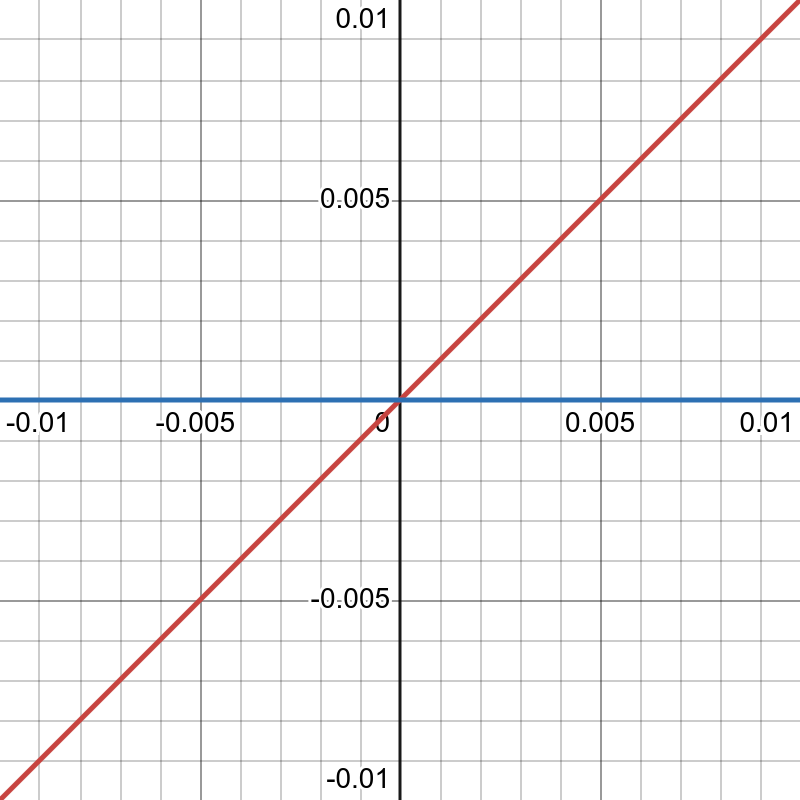
\includegraphics[height=0.3\textheight]{x_graph.png}
        \caption{The graph of $f(x) = x$ near $x = 0$}
      \end{figure}
    \end{column}
    \begin{column}{0.48\textwidth}
      \pause
      \begin{figure}
        \centering
        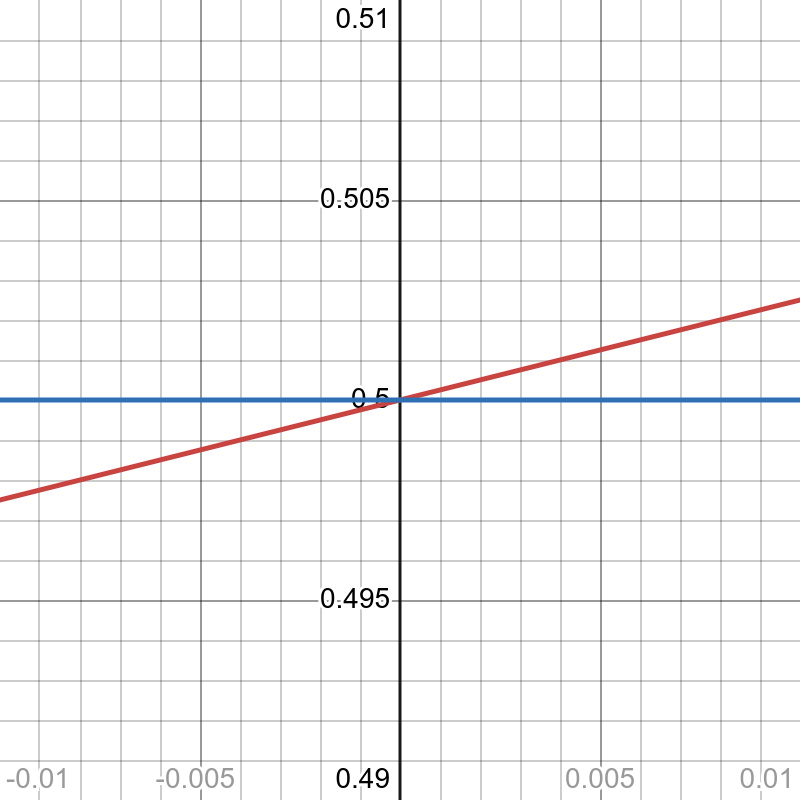
\includegraphics[height=0.3\textheight]{logistic_graph.png}
        \caption{The graph of a logistic function near $x = 0$}
      \end{figure}
    \end{column}
  \end{columns}
\end{frame}

\begin{frame}
  \frametitle{What to do?}

  So if constant functions $y = f(a) \approx f(x)$ don't approximate well enough \pause what's the next most complicated type of function we could approximate $f(x)$ by? \pause

  \textit{A linear function!}
\end{frame}

\section{The Derivative}

\begin{frame}
  \frametitle{Linear Approximation}

  We will introduce the (extremely \textit{extremely} important) concept of 
  the derivative via \textit{linear approximations}. \pause

  \begin{alertblock}{Goal}
    Find the linear function $\mathscr{L}(x) = mx + b$ that 
    ``\textit{best}" approximates the function $f(x)$ \pause 
    when $x \approx a$ for some fixed value $a$. \pause
  \end{alertblock}

  Why? \pause Oftentimes for scientific/engineering purposes,
  the actual functions that model complex phenomena \pause
  (like pendulum forces, population growth rates, reaction rates, etc) \pause
  are so wildly complicated that we cannot effectively study their true form. \pause

  However, taking their linear approximation \pause (since linear functions are exactly specified by a finite amount of data [the slope and the intercept, e.g.]) \pause
  often both simplify calculations vastly \textit{AND} approximate real world measurements well enough.
\end{frame}

\begin{frame}
  \frametitle{Best Linear Approximation I}

  (Aside: \pause Because we want to look at behavior when $x \approx a$,
  I'll switch to \textit{point-slope form} $\mathscr{L}(x) = m(x - a) + b$) \pause

  Idea 1: \pause We'll say that $\mathscr{L}(x) = m(x - a) + b$ is the 
  best linear approximation of $f(x)$ near $x = a$ \pause
  if $\lim\limits_{x \rightarrow a} \mathscr{L}(x) = \lim\limits_{x \rightarrow a} f(x)$. 
  \pause Pros/Cons? 
  \pause This at least forces \pause $b = \lim\limits_{x \rightarrow a} f(x)$.

  Idea 2: \pause ... if the error term $|f(x) - \mathscr{L}(x)| \rightarrow 0$ as $x \rightarrow a$. \pause But this is just the last idea dressed in a different hat... \pause

  We can't \textit{just} make conditions on limits of errors since 
  \pause the information about the linear term $m(x - a)$ ``\textit{dies}" as $x \rightarrow 0$.
\end{frame}

\begin{frame}
  \frametitle{Best Linear Approximation II}

  Solution: The error $|f(x) - \mathscr{L}(x)|$ should ``die" to $0$ faster than $|x - a|$ ``dies" to 0. \pause

  \begin{block}{Best Linear Approximation}\index{best linear approximation}
    A linear function $\mathscr{L}(x) = m(x - a) + b$ is the \textit{best linear approximation} to a function $f(x)$ at $x = a$ if: \pause
    \begin{equation}
      \lim\limits_{x \rightarrow a} \dfrac{|f(x) - \mathscr{L}(x)|}{|x - a|} = 0
    \end{equation} \pause
  \end{block}

  That's great and all - but how do we \textit{find} the best linear approximation?
\end{frame}

\begin{frame}
  \frametitle{Best Linear Approximation III}
  \begin{alertblock}{Determining the Best Linear Approximation}\index{best linear approximation!determining coefficients}
    Given a function $f(x)$, if a best linear approximation 
    $\mathscr{L}(x) = m(x - a) + b$ exists
    to $f(x)$ at $x = a$ then the following must be true: \pause
    \begin{enumerate}
      \item $b = \lim\limits_{x \rightarrow a} f(x)$ \pause
      \item $f(x)$ is continuous at $x = a$, so \pause
        \begin{equation}
          b = \lim\limits_{x \rightarrow a} f(x) = f(a)
        \end{equation} \pause
      \item We have the following expression for the slope $m$:
        \begin{equation}
          m = \lim\limits_{x \rightarrow a} \dfrac{f(x) - f(a)}{x - a}
        \pause = \lim\limits_{h \rightarrow 0} \dfrac{f(a + h) - f(a)}{h}
          \pause = IV_{x = a}(f(x))
        \end{equation}
    \end{enumerate}
  \end{alertblock}
\end{frame}

\begin{frame}
  \frametitle{The Derivative}
  Because this quantity has shown up sooooo many times, we give it a special name: \pause

  \begin{block}{Derivative of a function at a point}\index{derivative}\index{derivative!limit definition}
    The derivative of a function $f(x)$ at a point $x = a$, denoted $f'(a)$ \pause
    is the common value of the following four (equal) quantities: \pause
    \begin{enumerate}
      \item \begin{equation} \label{eq:derivative} f'(a) = \lim_{x \rightarrow a} \dfrac{f(x) - f(a)}{x - a} = \lim_{h \rightarrow 0} \dfrac{f(a + h) - f(a)}{h} \end{equation} \pause
      \item The slope of the best linear approximation to $f(x)$ at $x = a$. \pause
      \item The slope of the \textit{tangent} line to the graph of $y = f(x)$ at $x = a$. \pause
      \item The instantaneous velocity of a particle with position described by $f(x)$ at time $x = a$.
    \end{enumerate}
  \end{block}
\end{frame}

\begin{frame}
  \frametitle{Computing The Derivative}
  We often use \autoref{eq:derivative} to compute the derivative, \pause
  which is why we spent the first two weeks going over limits in such depth! \pause

  E.g. let's compute the derivative of the function $f(x) = x^2$ at $x = 2$! \pause

  \begin{columns}
    \begin{column}{0.48\textwidth}
      \begin{align}
        f'(2) &= \pause \lim\limits_{x \rightarrow 2} \dfrac{f(x) - f(2)}{x - 2} \pause \\
              &= \lim\limits_{x \rightarrow 2} \dfrac{x^2 - 2^2}{x - 2} \pause \\
              &= \lim\limits_{x \rightarrow 2} \dfrac{(x - 2)(x + 2)}{x - 2} \pause \\
              &= \lim\limits_{x \rightarrow 2} x + 2 \pause = 2 + 2 = 4 \pause
      \end{align}
    \end{column} 
    \begin{column}{0.48\textwidth}
      \begin{align}
        f'(2) &= \pause \lim\limits_{h \rightarrow 0} \dfrac{f(2 + h) - f(2)}{h} \pause \\
              &= \lim\limits_{h \rightarrow 0} \dfrac{(2 + h)^2 - 2^2}{h} \pause \\
              &= \lim\limits_{h \rightarrow 0} \dfrac{4 + 4h + h^2 - 4}{h} \pause \\
              &= \lim\limits_{h \rightarrow 0} \dfrac{4h + h^2}{h} \pause \\
              &= \lim\limits_{h \rightarrow 0} 4 + h \pause = 4 + 0 = 4
      \end{align}
    \end{column}
  \end{columns}
\end{frame}

\begin{frame}
  \frametitle{Interpreting the Derivative}
  Does this actually give the slope of the best linear approximation/tangent line? \pause 

  \begin{columns}[t]
    \begin{column}{0.48\textwidth}
      \pause
      \begin{figure}
        \centering
        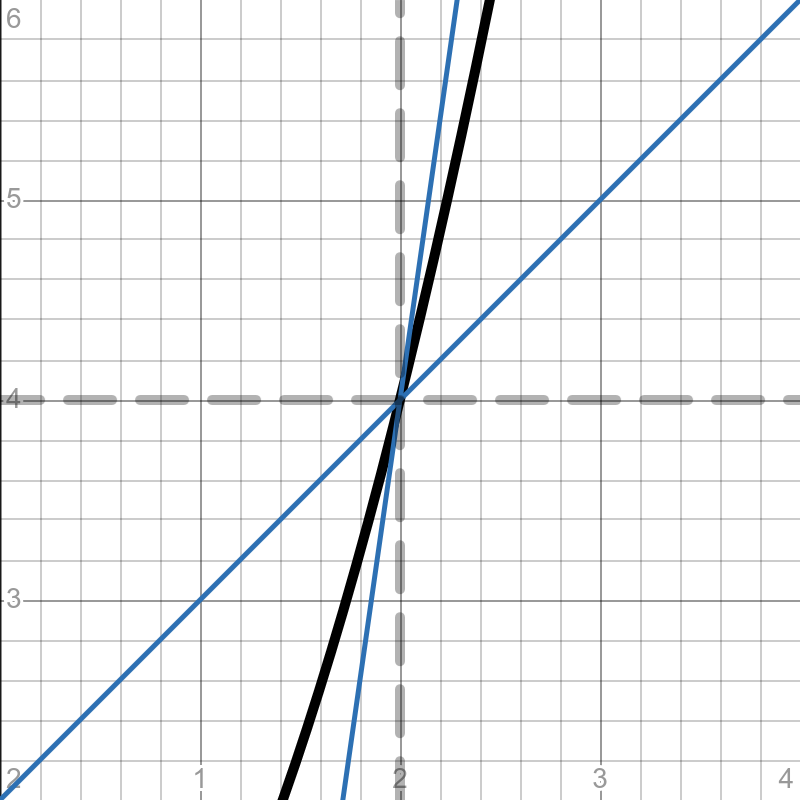
\includegraphics[height=0.3\textheight]{lin_approx_1_7.png}
        \caption{Linear approximations of $f(x) = x^2$ around $x = 2$ with slopes $m = 1,7$}
      \end{figure}
    \end{column}
    \begin{column}{0.48\textwidth}
      \pause
      \begin{figure}
        \centering
        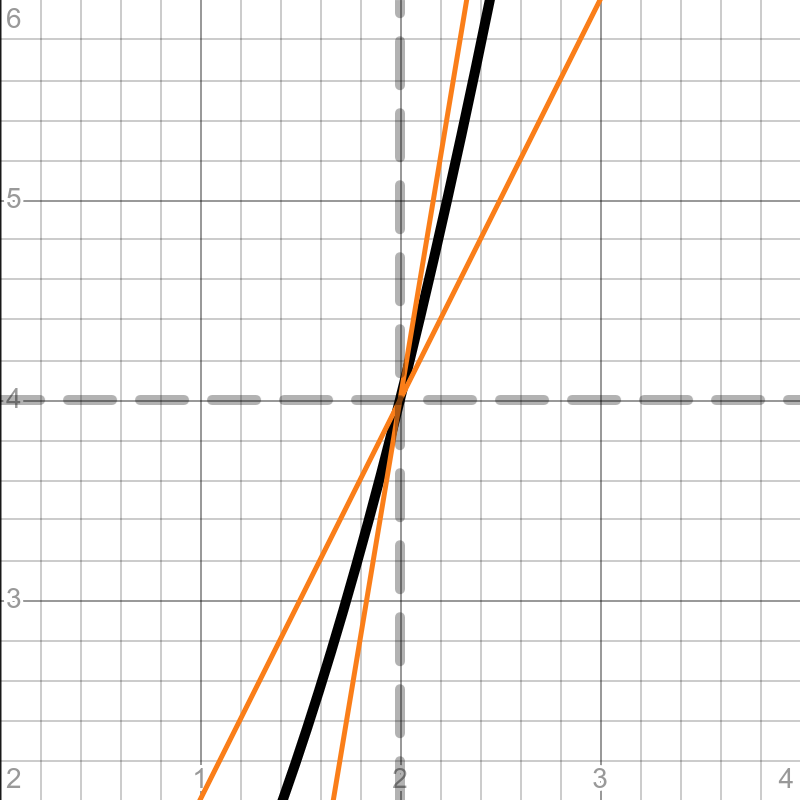
\includegraphics[height=0.3\textheight]{lin_approx_2_6.png}
        \caption{Linear approximations of $f(x) = x^2$ around $x = 2$ with slopes $m = 2,6$}
      \end{figure}
    \end{column}
  \end{columns}
  % ---- bottom row ----
  \begin{columns}[t]
    \begin{column}{0.48\textwidth}
      \pause
      \begin{figure}
        \centering
        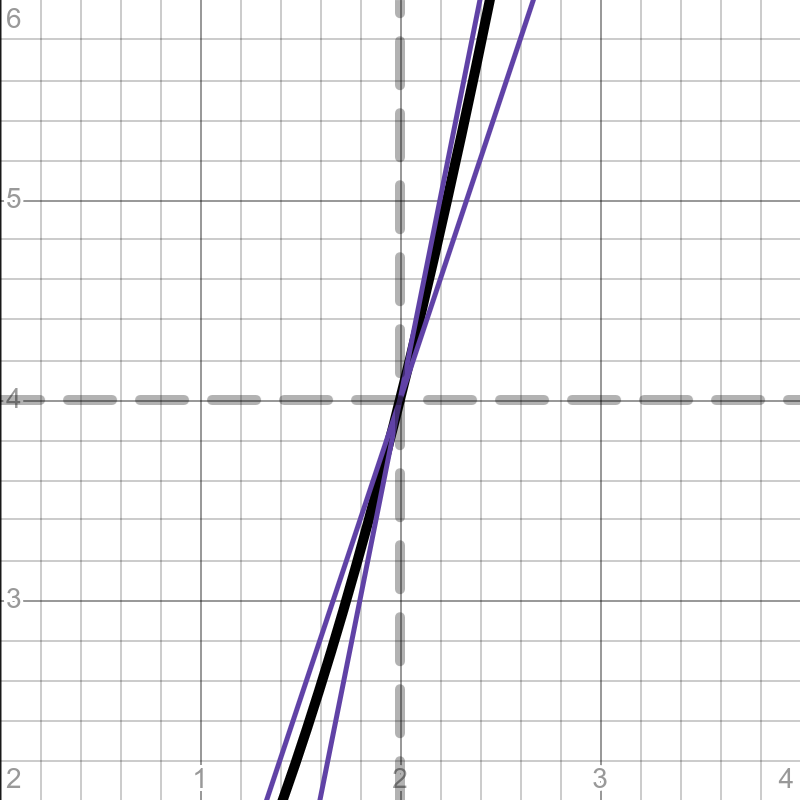
\includegraphics[height=0.3\textheight]{lin_approx_3_5.png}
        \caption{Linear approximations of $f(x) = x^2$ around $x = 2$ with slopes $m = 3,5$}
      \end{figure}
    \end{column}
    \begin{column}{0.48\textwidth}
      \pause
      \begin{figure}
        \centering
        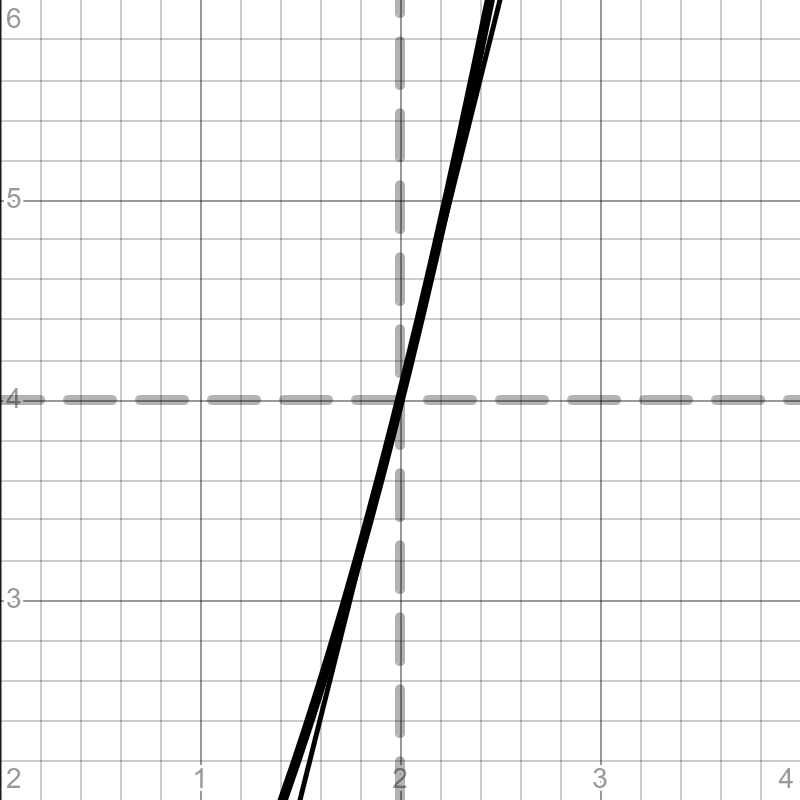
\includegraphics[height=0.3\textheight]{best_lin_approx.png}
        \caption{The best linear approximation of $f(x) = x^2$ around $x = 2$ with slope $m = f'(2) = 4$.}
      \end{figure}
    \end{column}
  \end{columns}
\end{frame}

\begin{frame}
  \frametitle{Computing the Derivative II}
  Let's try another one! \pause Let's compute $f'(4)$ when $f(x) = \sqrt{x}$. \pause

  \begin{columns}
    \begin{column}{0.48\textwidth}
      \begin{align}
        f'(4) &= \pause \lim \limits_{x\rightarrow 4} \dfrac{f(x) - f(4)}{x - 4} \pause \\
              &= \lim\limits_{x \rightarrow 4} \dfrac{\sqrt{x} - \sqrt{4}}{x - 4} \pause \\
              &= \lim\limits_{x \rightarrow 4} \dfrac{\sqrt{x} + \sqrt{4}}{\sqrt{x} + \sqrt{4}} \dfrac{\sqrt{x} - \sqrt{4}}{x - 4} \pause \\
              &= \lim\limits_{x \rightarrow 4} \dfrac{(\sqrt{x})^2 - (\sqrt{4})^2}{(x - 4)(\sqrt{x} + \sqrt{4})} \pause \\
              &= \lim\limits_{x \rightarrow 4} \dfrac{x - 4}{(x - 4)(\sqrt{x} + \sqrt{4})} \pause \\
              &= \lim\limits_{x \rightarrow 4} \dfrac{1}{\sqrt{x} + \sqrt{4}}
              \pause = \dfrac{1}{\sqrt{4} + \sqrt{4}} \pause = \dfrac{1}{4} \pause
      \end{align}
    \end{column}
    \begin{column}{0.48\textwidth}
      \begin{align}
        f'(4) &= \pause \lim \limits_{h \rightarrow 0} \dfrac{f(4 + h) - f(4)}{h} \pause \\
              &= \lim \limits_{h \rightarrow 0} \dfrac{\sqrt{4 + h} - \sqrt{4}}{h} \pause \\
              &= \lim \limits_{h \rightarrow 0} \dfrac{(4 + h) - 4}{(\sqrt{4 + h} + \sqrt{4})h} \pause \\
              &= \lim \limits_{h \rightarrow 0} \dfrac{h}{(\sqrt{4 + h} + \sqrt{4}) h} \pause \\
              &= \lim \limits_{h \rightarrow 0} \dfrac{1}{\sqrt{4 + h} + \sqrt{4}} \pause = \dfrac{1}{4}
      \end{align}
    \end{column}
  \end{columns}
\end{frame}
\begin{frame}
  \frametitle{Computing the Derivative III}
  For one last one, let's compute $f'(0)$ when $f(x) = | x|$. \pause
  \begin{align}
    f'(0) &= \pause \lim \limits_{x \rightarrow 0} \dfrac{f(x) - f(0)}{x - 0} \pause \\
          &= \lim \limits_{x \rightarrow 0} \dfrac{|x|}{x} \pause \\
          &\text{since $|x|$ is defined piecewise, let's look at one-sided limits:} \pause \\
    \lim_{x \rightarrow 0^{+}} \dfrac{|x|}{x} &= \lim_{x \rightarrow 0^{+}} \dfrac{x}{x} \pause \\
                                              &= \lim_{x \rightarrow 0^{+}} 1 \pause = 1 \pause \\
    \lim_{x \rightarrow 0^{-}} \dfrac{|x|}{x} &= \lim_{x \rightarrow 0^{-}} \dfrac{-x}{x} \pause \\
                                              &= \lim_{x \rightarrow 0^{-}} -1 \pause = -1 \pause
  \end{align}
  Since $\lim\limits_{x \rightarrow 0^{+}} \dfrac{f(x) - f(0)}{x - 0} \neq \lim\limits_{x \rightarrow 0^{-}} \dfrac{f(x) - f(0)}{x - 0}$ \pause
  this means that $f'(0)$ \textit{does not exist} \pause
  and there is \textit{\textbf{NO}} best linear approximation to $|x|$ around $x = 0$.
\end{frame}

\begin{frame}
  \frametitle{Differentiable Functions I}

  \begin{block}{Differentiable Function}\index{differentiable function}
    A function $f(x)$ is \textit{differentiable} at $x = a$ if any of the following equivalent conditions hold: \pause
    \begin{enumerate}
      \item The limit 
        \begin{equation}
          f'(a) = \lim\limits_{x \rightarrow a} \dfrac{f(x) - f(a)}{x - a} = \lim\limits_{h \rightarrow 0} \dfrac{f(a + h) - f(a)}{h}
        \end{equation} exists. \pause
      \item There exists a best linear approximation $\mathscr{L}(x) = f(a) + f'(a)(x - a)$ to $f(x)$ around $x = a$. \pause
      \item There is a unique tangent line to the graph of $y = f(x)$ at $x = a$.
    \end{enumerate}
  \end{block}
\end{frame}

\begin{frame}
  \frametitle{Differentiable Functions II}
  The two classes of functions we've defined so far 
  \pause (continuous \& differentiable) \pause
  are related in the following manner: \pause

  \begin{alertblock}{Continuity and Differentiability}\index{differentiable function!is continuous}\index{continuous function!from differentiable functions}
    For a function $f(x)$ and a point $x = a$ we have the following (equivalent) relationships: \pause
    \begin{enumerate}
      \item If $f(x)$ is differentiable at $x = a$ \pause
        then it \textit{must} be the case \pause 
        that $f(x)$ is also continuous at $x = a$. \pause
      \item If $f(x)$ is \textit{not} continuous at $x = a$ \pause
        then it \textit{can never} also be the case \pause
        that $f(x)$ is also differentiable at $x = a$.
    \end{enumerate}
  \end{alertblock}
\end{frame}

\begin{frame}
  \frametitle{Intuition for Continuity/Differentiability}
  The following intuition may be useful:

  \begin{alertblock}{Intuition for Continuity and Differentiability}
    \index{continuous function!intuition}\index{differentiable function!intuition}\index{intuition!for continuous functions}\index{intuition!for differentiable functions}
    We can intuitively recognize continuity/differentiability of a function $f(x)$ at a point $x = a$ from its graph as: \pause
    \begin{enumerate}
      \item continuity: if you can draw the graph of $f(x)$ near $x = a$ \textit{without} lifting up your pencil \pause (no jump discontinuities) \pause or without rapidly oscillating it \pause (no $\sin(\dfrac{1}{x})$) \pause
      \item differentiability: if the graph of $f(x)$ ``locally looks like" the graph of a linear function near $x = a$ \pause i.e. the function is both continuous and does not make any sharp changes near $x = a$.
    \end{enumerate}
  \end{alertblock}
\end{frame}

\begin{frame}
  \frametitle{Terminological Potpourri I}

  There's a lot of terminology so here's some scattered parts that didn't fit nicely. \pause

  \begin{block}
    {Tangent Line}\index{tangent line}\index{tangent line!equation of}
    Given a function $f(x)$ and a point $x = a$, \pause 
    the \textit{tangent line} to $f(x)$ at $x = a$ is the line that: \pause
    \begin{enumerate}
      \item intersects the graph of $y = f(x)$ at $(a, f(a))$ \pause
      \item but does not \textit{cross} the graph at that point \pause (e.g. it just ``glances" off). \pause
    \end{enumerate}

    The tangent line \textit{is} the graph of the best linear approximation to $f(x)$ at $x = a$, \pause
    as such the equation of the tangent line, for $f(x)$ differentiable at $x = a$, is: \pause
    \begin{equation}
      y = f(a) + f'(a)(x - a).
    \end{equation} \pause
  \end{block}
\end{frame}
\begin{frame}
  \frametitle{Terminological Potpourri II}
  \begin{block}{Units of the Derivative}
    If our function represents the relationship between \pause
    an input quantity $x$ measured in units of $U_{in}$ \pause
    and an output quantity $f(x)$ measured in units of $U_{out}$ \pause
    the derivative $f'(a)$ (if it exists) \pause
    is measured in units of $\frac{U_{out}}{U_{in}}$. \pause
  \end{block}

  E.g. if $s(t)$ is the distance in miles that a car travels, where $t$ is the time since starting measured in hours, \pause
  $s'(t) = v(t)$ is the velocity and is measured in units of miles per hour.
\end{frame}

\begin{frame}
  \frametitle{Worksheet Time!}
  Let's get into groups and work on the worksheet!
\end{frame}

\begin{frame}
  \frametitle{End of Class!}
  That's all folks!
\end{frame}
\end{document}
